\documentclass{article}

\usepackage[utf8]{inputenc}
\usepackage[T1]{fontenc}
\usepackage{fancyvrb}

\usepackage{Sweave}
\begin{document}
\Sconcordance{concordance:train_perceptron.tex:train_perceptron.Rnw:%
1 6 1 1 0 16 1 1 3 1 0 1 1 2 2 2 1 1 2 4 1 1 2 3 1 4 0 1 2 4 1 1 2 1 0 %
4 1 3 0 1 2 10 1 1 2 1 0 1 1 2 2 1 9 7 0 1 2 4 1 4 0 1 2 2 1 1 3 6 0 1 %
2 1 1}


\title{Treinamento Perceptron Simples}
\author{Matheus Araujo - 2013066265}
\date{}

\maketitle

\section{Treinamento Perceptron Simples}

Nessa atividade, a técnica de \emph{Perceptron Simples} será aprimorada através de treinamento. Em vez de usarmos pesos calculados para o vetor de pesos da Rede Neural, eles serão calculados por uma função de treinamento.

\subsection{Geração de dados}

Inicialmente, os dados são gerados conforme o código a seguir:

\begin{Schunk}
\begin{Sinput}
>   rm(list = ls())
>   library('plot3D')
>   source('treinap.R')
>   s1<-0.4
>   s2<-0.4
>   nc<-200
>   xc1<-matrix(rnorm(nc*2),ncol=2)*s1 + t(matrix((c(2,2)),ncol=nc,nrow=2))
>   xc2<-matrix(rnorm(nc*2),ncol=2)*s2 + t(matrix((c(4,4)),ncol=nc,nrow=2))
>   plot(xc1[,1],xc1[,2],col='red',xlim=c(0,6),ylim=c(0,6),xlab='x_1',ylab='x_2')
>   par(new=T)
>   plot(xc2[,1],xc2[,2],col='blue',xlim=c(0,6),ylim=c(0,6),xlab='',ylab='')
>   x1_reta<-seq(6/100,6,6/100)
>   x2_reta<- -x1_reta+6
>   par(new=T)
>   plot(x1_reta,x2_reta,type='l',col='orange',xlim=c(0,6),ylim=c(0,6),xlab='',ylab='')
\end{Sinput}
\end{Schunk}
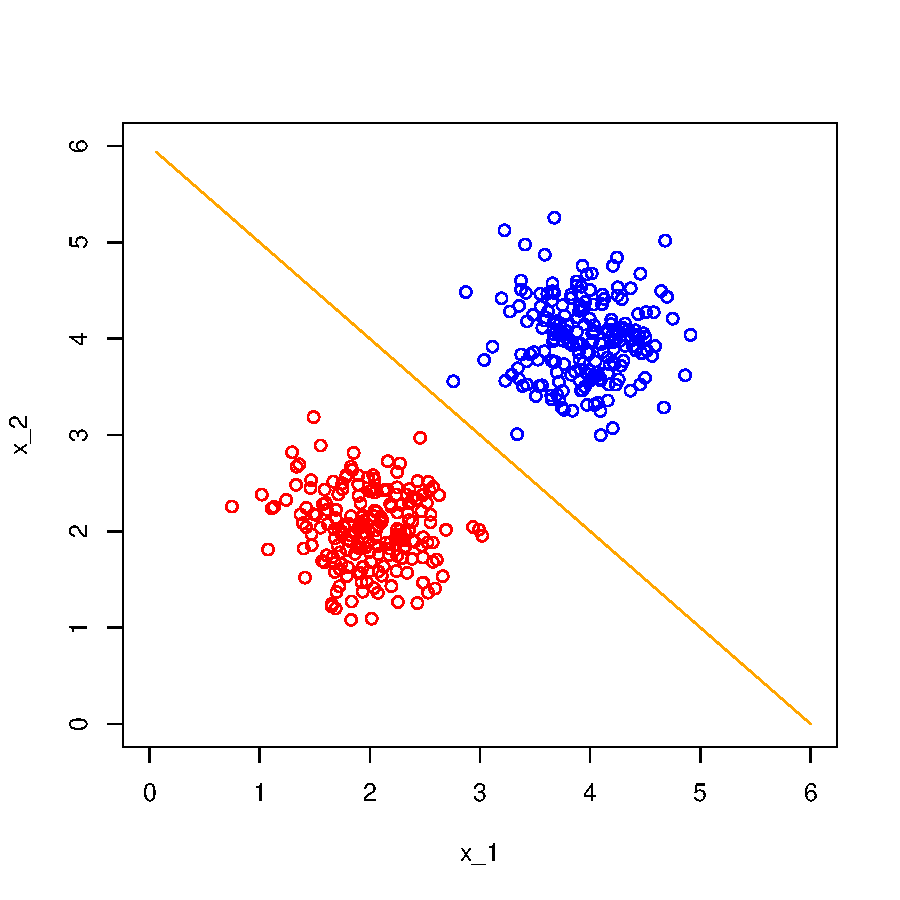
\includegraphics{train_perceptron-001}

\subsection{Treinamento}

Agora os valores para o vetor de pesos são calculados pela função \emph{treinap} no arquivo \emph{treinap.R}.

\begin{Schunk}
\begin{Sinput}
>   X = rbind(xc1,xc2)
>   yc1<-matrix(0,nrow=nc,ncol=1)
>   yc2<-matrix(1,nrow=nc,ncol=1)
>   yd<-rbind(yc1,yc2)
>   w = treinap(X, yd, 0.1, 0.01, 100, 1)
\end{Sinput}
\end{Schunk}

\subsection{Função de treinamento}

A função \emph{treinap} é apresentada a seguir:

\VerbatimInput{treinap.R}

\subsection{Resultados}

O resultado da função de treinamento é mostrado a seguir:

\begin{Schunk}
\begin{Sinput}
>   seqi<-seq(0,6,0.1)
>   seqj<-seq(0,6,0.1)
>   M<-matrix(0,nrow=length(seqi),ncol=length(seqj))
>   ci<-0
>   for(i in seqi) {
+     ci<-ci+1
+     cj<-0
+     for(j in seqj) {
+       cj<-cj+1
+       M[ci,cj]<-1*(i*w[[1]][2]+j*w[[1]][3]>=w[[1]][1])
+     }
+   }
>   plot(xc1[,1],xc1[,2],col='red',xlim=c(0,6),ylim=c(0,6),xlab='x_1',ylab='x_2')
>   par(new=T)
>   plot(xc2[,1],xc2[,2],col='blue',xlim=c(0,6),ylim=c(0,6),xlab='',ylab='')
>   par(new=T)
>   contour(seqi,seqj,M,xlim=c(0,6),ylim=c(0,6),xlab='',ylab='')
\end{Sinput}
\end{Schunk}
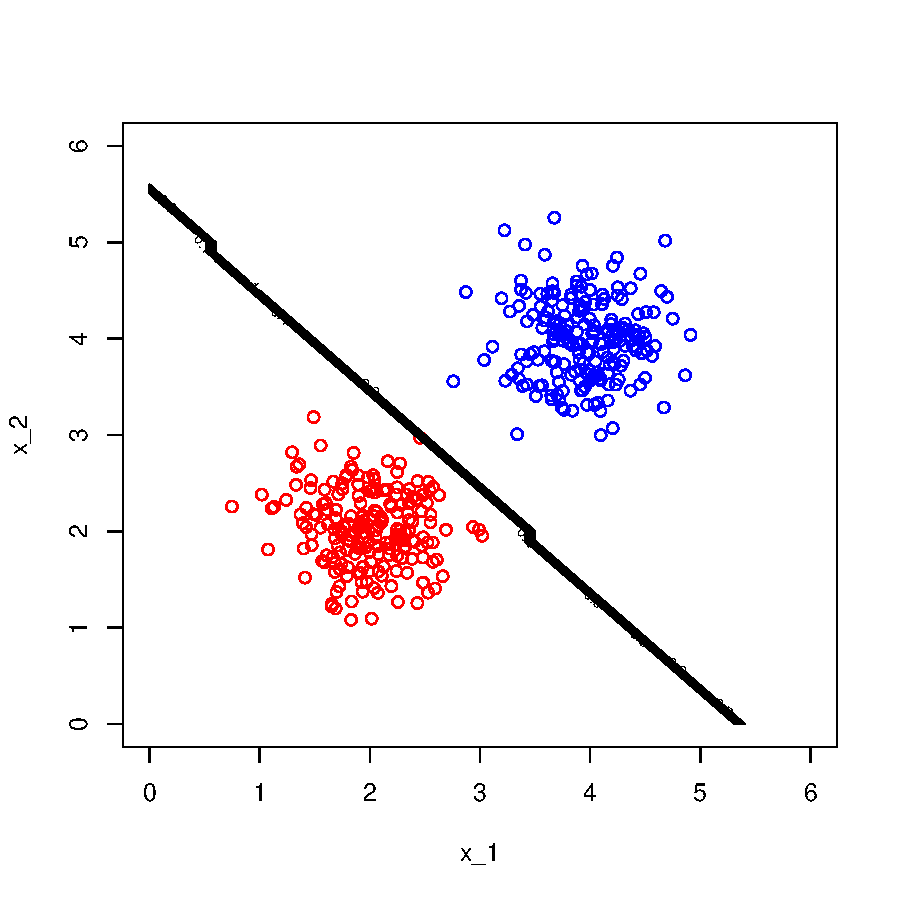
\includegraphics{train_perceptron-003}

Visão em 3D:

\begin{Schunk}
\begin{Sinput}
>     persp3D(seqi,seqj,M,counter=T,theta=55,phi=30,r=40,d=0.1,expand=0.5,ltheta=90,
+             lphi=180,shade=0.4,ticktype="detailed",nticks=5)
\end{Sinput}
\end{Schunk}
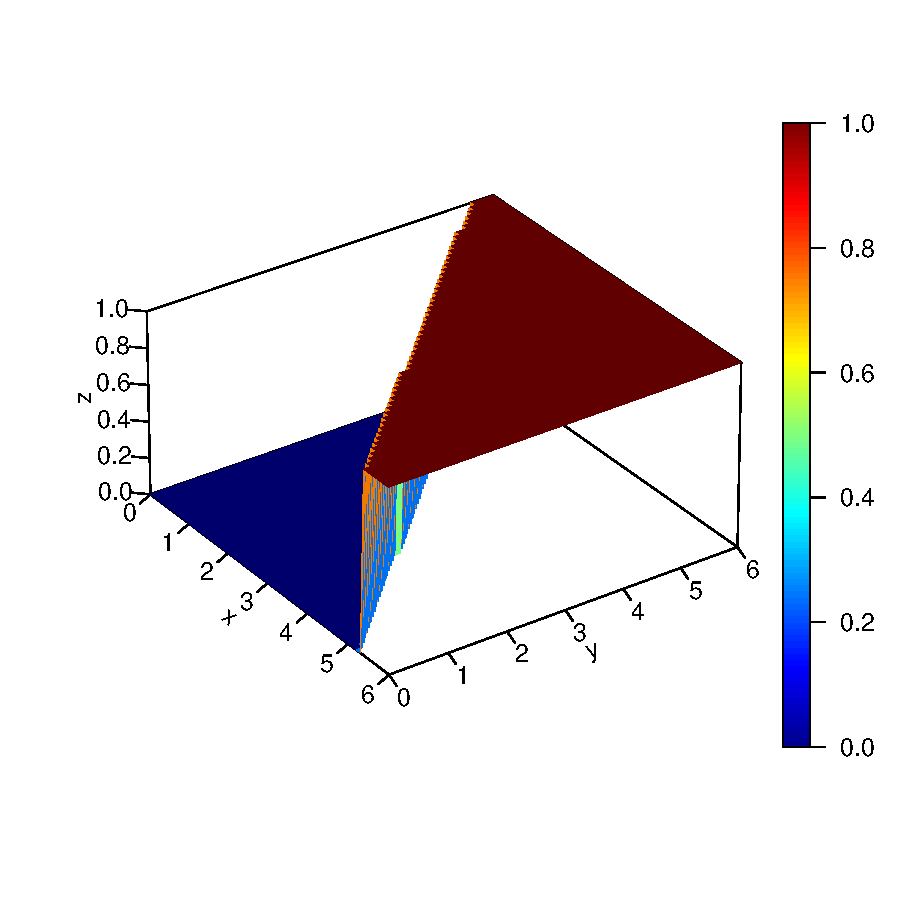
\includegraphics{train_perceptron-004}

\end{document}
